\documentclass[../main.tex]{subfiles}

\begin{document}

\chapter{Không làm được thơ là coi như thất bại}

\begin{metadata}

\begin{flushright}21.5.2008\end{flushright}

Hoàng Hưng

Nguồn: Tạp chí Doanh nhân Sài Gòn cuối tuần 16/5/2008

\end{metadata}

\begin{multicols}{2}

\begin{figure}
	\centering
	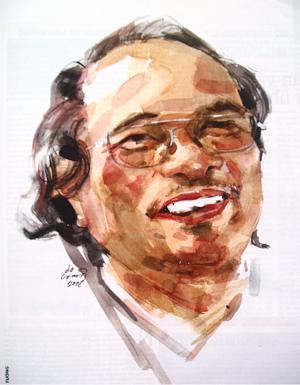
\includegraphics[width=\textwidth]{../img/tho210508.jpg}
	\caption{Nhà thơ Hoàng Hưng, ký hoạ của Hoàng Tường}
\end{figure}
 Nhà thơ Hoàng Hưng được biết đến như một điển hình của ý thức cách tân rốt ráo. Trên xa lộ chữ nghĩa, hành giả Hoàng Hưng mải miết xây một lối riêng bằng những từ, ngữ vuông vức, gắn kết bền chặt, đầy sức mạnh của tư duy, chiêm nghiệm, suy tưởng... Tập thơ \textit{Hoàng Hưng - 36 bài thơ} (do Nhà xuất bản Nghệ An và Trung tâm Văn hoá Ngôn ngữ Đông Tây ấn hành quý I năm 2008) với những bài thơ cũ và mới: “Người yêu miệt biển”, “Cửa sông”, “Người đi tìm mặt”, “Tuyết Sơn”, “Nghe”... đã làm sống lại từng chặng đường thơ đầy gai góc, va xiết của ông. Chúng tôi đã gặp nhà thơ Hoàng Hưng và nghe ông chia sẻ nhiều hơn về hành trình thơ.  
 
\textit{Đọc thơ ông, người ta sẽ nghĩ ông có một vẻ bề ngoài dữ dội, một tính cách kì dị thế nào đấy…} 
 
Đúng đấy, nhiều người thất vọng khi gặp tôi. Đọc thơ thôi, nhất là tập \textit{Ngựa biển,} họ nghĩ tôi trông phải hoành tráng, dữ dội, ngang tàng lắm. Không ai nghĩ trông tôi lại có vẻ cù lần thế này. Tính cách thực của con người nhiều lúc không thể hiện ra bên ngoài để cho các nhà “tướng mạo học” bắt được đâu. 
 
\textit{Ông đã đến với thơ như thế nào? Vì sao thơ ông lại có sự ảnh hưởng từ các trào lưu thơ phương Tây đậm nét như vậy?} 
 
Tôi học tiếng Pháp từ bé. Bố tôi là một trong số các bác sĩ y khoa đầu tiên đầu tiên học ở Pháp về nên nhà tôi rất nhiều sách Pháp. Mười tuổi tôi đã bắt đầu dịch thơ Pháp rồi. Học lớp nhất (lớp 4, lớp 5 bây giờ) ngồi trong lớp tôi dịch những bài thơ trong sách giáo khoa Pháp văn. Cũng làm mấy bài thơ đăng trên trang thơ “Thiếu nhi” của \textit{Nhật báo Giang Sơn}. Nhưng hồi đó tôi chỉ dịch và làm thơ một cách hồn nhiên, không nghĩ mình lại đeo đuổi thơ đến suốt cuộc đời.  
 
Ý thức một cách nghiêm túc về thơ của tôi đến sau đó không lâu. Học cấp hai thì đã cảm thấy là mình phải đi theo con đường ấy. Đến cấp ba thì coi như đã xong xuôi, tôi đã quyết định học đại học ngành ngữ văn. Tôi vào khoa Văn trường Đại học Sư phạm Hà Nội, tuy nhiên chưa học ngày nào thì có lời kêu gọi học sinh đi Tây Bắc dạy học cho quân đội, máu giang hồ nổi lên, thế là tôi đi luôn. Đi để làm thơ đấy. Nhà thơ Phạm Hổ chính là người mang thơ của tôi về Hà Nội đăng báo \textit{Văn Nghệ}. Hai năm sau tôi về Hà Nội, lại thi vào khoa Văn học tiếp, học vào loại xuất sắc đấy! 
 
Bài thơ “Gửi anh” mà bây giờ nhiều người vẫn còn nhắc đoạt giải cuộc thi do báo \textit{Văn Nghệ} tổ chức năm 1965. Nói chung lúc đầu thơ tôi cũng chỉ theo tình cảm hồn nhiên. Nhưng như tôi đã nói, tôi ngày càng chịu ảnh hưởng sâu của văn hóa phương Tây, đặc biệt là tinh thần tự do cá nhân và thẩm mỹ hiện đại. Bước ngoặt là sau khi ra trường, từ năm 1965 đến năm 1973 tôi dạy học ở Hải Phòng lúc đó là thành phố công nghiệp, thành phố hải cảng, nó có một không khí phóng khoáng mạnh mẽ mà tôi rất mê. Tôi có một anh bạn họa sĩ ở đó, anh có rất nhiều sách về hội họa hiện đại phương Tây. Tôi đọc và vỡ ra nhiều thứ. Tôi có thêm nhiều kiến thức và hơn hết là tinh thần khám phá, phiêu lưu về nghệ thuật!  
 
Tuy nói là ảnh hưởng phương Tây nhưng ra tôi không ảnh hưởng cụ thể của ai, dù tôi rất thích và đã dịch thơ của Lorca, của Apollinaire. Có lẽ tôi chỉ ảnh hưởng cái tinh thần thôi! 
  
\textit{Chuyện “bếp núc” thơ  của các nhà thơ luôn có nhiều điều thú vị, vì nó mang những quan niệm sáng tác riêng của mỗi người. Với ông, các “món” thơ được làm thế nào?} 
 
Cái gì sẽ thành thơ? Thật khó nói. Trời sinh ra anh nhà thơ có rung cảm thơ. Cùng một thực tế, người bình thường không để ý nhưng anh nhà thơ lại có rung cảm. Một làn gió, một trận mưa cũng đủ làm nhà thơ tuôn trào câu chữ. Tuy nhiên đó chỉ là cái cớ. Trong nhà thơ phải chất chứa đầy, phải có sẵn (tri thức, kinh nghiệm, suy ngẫm, câu chữ) rồi mới ra thơ được. Xúc cảm bất chợt giống như mồi lửa bắt cháy những chất cháy có ở trong mình.  
 
Có người cho rằng cứ chịu khó viết hàng ngày rồi thơ sẽ ra. Tôi không làm được thế nên làm không đều và không nhiều được, và tôi cũng không cho thế là hay. Theo tôi thơ phải là tinh chất, có người cả đời mới chắt ra được vài câu thơ hay, có người cả đời vẫn là nhà thơ của chỉ một bài thơ. Tôi cho rằng nhà thơ khi chết có khoảng 10 bài người ta nhớ đến là hạnh phúc lắm rồi. Xem ra quan niệm ấy lại khá cổ điển, so với quan niệm phổ biến ở phương Tây hiện đại coi thơ là một cách chế tạo, một “thuật giả kim” ngôn ngữ, việc làm thơ mang tính chuyên nghiệp cao. Nhưng tôi thú thực, nhiều nhà thơ thế giới có thể cho ra đời mỗi năm 1 tập, tôi đọc cũng chỉ thấy ở mỗi tập vài bài có chất lượng.  
  
\textit{Ông có những câu thơ trong tập thơ }Hành trình\textit{ mới đây rằng: }Vào xa lộ/ta tìm ta/ Rừng chữ/ Ta thấy ta rồi/ sằng sặc cười/nước mắt một đời/ đổi một dòng hư ảo/ thế thôi? (“Xa lộ thông tin”).\textit{ Phải chăng giữa xa lộ thông tin ngày hôm nay, cuộc đi tìm chữ khó khăn cho các nhà thơ hơn trước đây? Tìm chữ cũng là tìm mình, ông có tìm được mình không?} 
 
Xa lộ thông tin là một tình thế mới cho các nhà thơ của chúng ta. Trước đây họ đứng ở một góc rừng hẻo lánh, một cái ao con con, tưởng mình là nhất, nay họ bước ra ngoài gặp xa lộ thông tin mênh mông nên cảm thấy choáng ngợp. Rồi chợt nhận ra mình chỉ như một hạt bụi vô nghĩa, mất hay còn đều không quan trọng. Tôi đi tìm mình, cũng tìm được nhưng rồi cũng nhận ra mình bé nhỏ quá. Ví dụ nếu vào mạng gõ tên Hoàng Hưng để tìm kiếm, thì máy tính sẽ cho vài nghìn kết quả về nhà thơ Hoàng Hưng. Thế nhưng số lượng ấy vẫn là quá nhỏ trong hàng tỉ tỉ thông tin trên cái xa lộ rộng khủng khiếp này, và Hoàng Hưng chỉ là một hạt cát, biết có ai thèm để ý.  
 
\textit{Câu thơ của ông: }Mình hành khất gì đây / hành khất một niềm tin bên trên lý lẽ\textit{ là một câu thơ có nhiều suy ngẫm…} 
 
Niềm tin luôn là vấn đề lớn trong đời sống tâm linh con người. Thông thường người ta sống chỉ bằng lý lẽ, cái này đúng cái kia sai, dùng luận lý để nhận thức vấn đề và quyết định hành xử. Giờ thì thực tế chứng minh sự phân biệt trắng đen, đúng sai rạch ròi thật rất khó và xét đến cùng cũng là vô nghĩa. Niềm tin Phật giáo dựa trên nguyên lý: không phân biệt đúng sai, thiện ác, được mất… Nếu đạt được một niềm tin bên trên tất cả những thứ đó, tức là con người đã ngộ. Song chúng ta sống quá nặng về lý trí, nô lệ cho lý lẽ, khó mà thoát được. Thế nên khi tôi cảm thấy mình sai, tôi muốn hành khất để có được sự thanh thản ở trên tất cả, đó là niềm tin vào ngộ, vào sự giải thoát tuyệt đối. Tất nhiên đó chỉ là một cách nói trong lúc vẫn còn “mê”, chứ niềm tin, sự giải thoát không thể cầu xin ở bên ngoài được, chỉ tự mình chứng nghiệm được thôi. 
 
\textit{Vậy thơ ông chịu ảnh hưởng Phật giáo từ khi nào?} 
 
Sau năm 75, tôi đọc nhiều sách Phật. Mới đọc tôi choáng váng và sốc! Đầu óc tôi chứa đầy những triết lý phương Tây nhưng hoá ra mọi thứ không như tôi vẫn ảo tưởng. Chùm thơ “Nhập môn” trong tập \textit{Người đi tìm mặt} mà nhiều người cho là tục tĩu với các từ như đờm, dãi, tinh khí… thực ra đều lấy chất liệu từ kinh Phật cả đấy. Lúc đó tôi rất hoang mang, chưa tìm được cảm giác bình yên bởi những thành lũy kiến thức, lối tư duy trong tôi đảo điên, đổ vỡ. Sau rồi tinh thần Thiền thấm dần vào thơ tôi và đến tập \textit{Hành trình} có lẽ tôi đã đạt được độ bình an nhất định, tôi thấy được những lẽ giản dị của cuộc đời. Cả tập thơ đó cũng được sắp xếp theo mức độ phát triển nhận thức. Ví dụ “Mưa Bangkok” còn lấn bấn, trăn trở, đến “Chó rừng” vẫn còn nỗi bất an, băn khoăn. “Tuyết sơn”, “Bên mái chùa” thì đã bình an trong bất an của thế sự, có trong cái không, còn trong cái mất.  
 
\textit{Trong các tập thơ trước của Hoàng Hưng còn thấy nhiều bóng dáng phụ nữ, đến tập thơ }Hành trình\textit{ mới nhất của ông thì thấy đi đâu hết cả...} 
 
Tôi không còn trẻ nữa. Hồi trẻ thơ tôi cũng thấp thoáng hình bóng những người con gái, nhưng gần đây thơ tôi chỉ nói về người vợ của mình. Đời tôi có nhiều bi kịch và vợ tôi chính là người sẻ chia, luôn ở bên tôi, là chỗ dựa của tôi. Tôi thấy nhiều người dễ yêu và dễ làm thơ tình, tôi không tin lắm vào tình ấy và thơ ấy. Tình yêu cũng như thơ không dễ dàng như vậy. Và thơ tình và thơ tán gái là hoàn toàn khác nhau.  
 
Trong thơ tôi, số lượng thơ tình chiếm không nhiều. Ngay cả khi còn trẻ tôi cũng không được coi là người nặng về thơ tình. Thơ tôi có những khát khao trừu tượng, những chuyện nhân gian thế sự rộng hơn… Nhiều bài thơ của tôi thoáng nhìn cứ tưởng thơ tình nhưng thực ra không hẳn thế. Ví dụ bài thơ “Người yêu miệt biển”, có bóng hình phụ nữ và tình yêu đấy nhưng sâu xa còn là những chiêm nghiệm về đời sống, là nỗi thất vọng lớn, là sự đổ vỡ… Tôi hay băn khoăn về lý tưởng sống. Lý tưởng sống là khát vọng tìm được chân lý, tìm được ý nghĩa thật sự của đời sống, sống thế nào để có một đời sống đẹp. Đó cũng là tôn giáo. Tìm tôn giáo là tìm lý tưởng sống thế nào cho có ý nghĩa, cho sự bất tử để chống lại sự hữu hạn của đời người.  
 
Thi ca, văn chương không có lý tưởng, không có niềm tin, không có tín ngưỡng thì nông choèn. Các tác phẩm lớn của phương Tây rất hướng thượng, bao giờ cũng có một cái gì mênh mông, cao lớn đằng sau câu chữ. Không giống như văn học Trung Quốc hoặc Việt Nam bây giờ, chỉ bày tất cả ra đó, trần trụi, sống sượng, kể cũng đã nhưng lắm lúc phát mệt. Cả \textit{Báu vật của đời} của Mạc Ngôn mà nhiều người khen rốt lại cũng vậy, tôi không thấy gì sâu sa, cao thượng toát lên từ tác phẩm đó.   
  
\textit{Ông Chu Văn Sơn trên báo }Công an Nhân dân\textit{ (đăng lại trên Phongdiep.net) nhận định: “Nhiều người cứ mải tìm kiếm ngoài mình, vì thế mà chưa đi vào được cái lõi của sự cách tân. Nhìn từ trường hợp nhà thơ Hoàng Hưng. Trước đây, anh là người say mê cách tân khá triệt để theo phương Tây. Nhưng đến tập }Hành trình\textit{ thì dù vẫn đầy yếu tố siêu thực nhưng lại rất gần gũi với truyền thống phương Đông. Đó là sự trở về chín chắn, cũng là tới bến của một hành trình sáng tạo”. Nghĩa là ông Chu Văn Sơn đánh giá rất cao tập }Hành trình\textit{ và tập thơ cũng đạt Giải thưởng Văn học năm 2006. Nhưng nhiều người lại cho rằng }Hành trình\textit{ không còn hấp dẫn như các tập trước đây, không bằng }Người đi tìm mặt\textit{. Ông nghĩ như thế nào? Phải chăng “chín chắn” và “tới bến” thì không hấp dẫn nữa?} 
 
Tôi cũng không rõ lắm, nhưng những người trẻ có thể không thích \textit{Hành trình} của tôi vì nó trầm đi nhiều. Họ thích những tập có sự cuồng nhiệt hay khắc khoải như \textit{Ngựa biển} hay là \textit{Người đi tìm mặt}. Song cũng có rất nhiều bạn bè tôi cho biết họ rất thích tập thơ này, rằng tập thơ này mới là đạt. Vậy là tôi may mắn. Thời kỳ nào cũng có một lượng độc giả nhất định. Còn độc giả thay đổi là điều hoàn toàn tất nhiên và hợp lẽ. Tôi cũng thay đổi chứ có đứng yên một chỗ đâu. Nhưng mà “tới bến” như ông Chu Văn Sơn nói thì còn lâu. Tuy rằng ông ấy có ý đánh giá cao thơ tôi thật nhưng mà tới bến, giác ngộ rồi thì thì tôi còn làm thơ làm gì nữa. Làm thơ là chưa ngộ phải đi tìm cái ngộ. Tôi vẫn đang làm thơ, đang đi tìm, mà ông ấy nói tôi tới bến rồi thì có khác gì… khai tử nhà thơ Hoàng Hưng! 
  
\textit{Nói chuyện với nhiều người ngoại đạo văn chương, họ biểu lộ thái độ không hề thiện cảm với thơ và danh hiệu nhà thơ. Nhạc sĩ: rất hay, nhà văn: cũng tạm được, nhưng nhà thơ… Với họ thơ thì phù phiếm, các nhà thơ bị coi là hoang tưởng, thường xuyên không có tiền. Và họ không hiểu vì sao có một số người cứ đi làm thơ. Ông nghĩ thế nào?} 
 
Thời đại này vị trí của thơ đã giảm đi. Trước đây sinh hoạt tinh thần không nhiều nên thơ mới có vị trí gần như độc tôn. Nhất là trong xã hội thực dụng bây giờ thì thơ lại càng mất giá. Nhà thơ sống bằng gì? Thơ là một hoạt động tinh thần thuần túy, người ta làm nhiều việc khác nhau để sống, còn làm thơ chỉ là thú vui, niềm đam mê riêng.  
 
Thắng thắn mà nói, thơ đúng nghĩa bây giờ chỉ dành cho một số người tinh hoa, chứ không phải cho đại chúng. Thứ thơ được phổ biến rộng rãi thì chỉ làm cho người đời rẻ rúng nhà thơ, có lẽ họ cho rằng làm thơ dễ lắm! Chỉ những người trong đạo mới hiểu giá trị của hai chữ “nhà thơ” (đúng nghĩa). Bởi vì làm thơ khó lắm. Nhà thơ phải có một bản năng thơ, do thiên phú, đầy bí ẩn, mà trường hợp Trần Đăng Khoa là tiêu biểu, chứ không phải học mà làm thơ được (hoặc những người có thiên phú thực ra đã học qua nhiều kiếp trước rồi chăng?). Không có cử nhân thơ hay tiến sĩ thơ. Vậy nên trong bảng xếp hạng của xã hội, người ta không biết xếp nhà thơ vào vị trí nào. Chỉ những người trong giới sáng tạo mới biết nhà thơ là danh hiệu quý vào loại nhất. Những người đã từng làm thơ rồi bỏ thơ chuyển sang viết lách nhiều thể loại khác, cuối cùng vẫn mong được gọi là nhà thơ.  
 
\textit{Trong các nhà thơ trẻ hiện nay, ông thích ai?} 
 
Tôi đang cảm thấy hoang mang trước thơ trẻ. Tôi cảm giác không còn bắt đuợc vào cái nhìn của họ nữa nên tôi không dám phán bừa. Lớp Phan Huyền Thư, Vi Thuỳ Linh, nhóm Mở Miệng, Lynh Bacardi... tôi thấy vẫn còn theo được, chứ bây giờ bảo tôi nói về thơ lớp trẻ hơn tôi cảm thấy không tự tin nữa. Cần có một lớp nhà phê bình trẻ hơn, ở gần họ hơn.  
 
\textit{Ông có khi nào thấy mệt mỏi trên hành trình thơ?} 
 
Làm thơ là sướng nhất, là hạnh phúc, sao lại nói là mệt. Mệt nhất chính là những lúc không làm được thơ. Đau khổ nhất là khi mình làm được mọi thứ nhưng không làm được thơ. Tôi cũng có nhiều khi như vậy, tôi nghi ngờ mình: hết thơ rồi chăng, không còn rung cảm, không còn hướng tới cái gì nữa chăng… Với người mê thơ thì chẳng có gì quan trọng hơn là làm thơ, không làm được thơ là đời mình coi như thất bại.  
 
\textit{Thơ với người này là một cuộc chơi, cuộc thử nghiệm, với người khác là tôn giáo, nhưng dù là gì thì người ta cũng có được và có mất. Vậy khi chơi với thơ, ông được gì và mất gì?} 
 
Với thơ, nói được mất là vô cùng. Nếu nhìn từ góc độ của người đời, họ sẽ cho là với năng lực và nỗ lực làm việc như tôi, tôi có thể đạt được nhiều thứ, vật chất, quyền lực, danh tiếng… Vào thơ là danh lợi đời thường mất rất nhiều. Chưa kể những tai nạn có thực và tiềm ẩn. Nhưng tôi không coi đó là mất. Được làm việc mình thích thì là được chứ, hạnh phúc chứ. Nên tôi cho là tôi được nhiều hơn. Sau rất nhiều gian lao, cuối cùng tôi vẫn có cuộc sống vật chất đầy đủ, lại có cơ hội đi nhiều nơi trên thế giới mà đều là nhờ thơ cả đấy. Tôi tự hào mình là một trong những nhà thơ tự do nhất, chưa bao giờ vì cái gì mà phải uốn bút. Tôi được quá nhiều. 
 
\textit{Xin cảm ơn ông!} 
\end{multicols}
\end{document}